\clearpage
\section{Implementing Single Shot Detector}
\subsection*{Task 4b}
As we have 10 000 images in the dataset, one can calculate the iterations by taking the size of the dataset, divided by batch size. 
For each epoch you iterate over all the batches. This means that with batch size 32, yielding 312 batches, the model need to converge at 75-77\% during 20 epochs. 
\begin{equation*}
    312 \cdot 20 = 6240
\end{equation*}
My implementation reached a mean average precision of 74\% during 6 000 iterations.
The two requested graphs, respectively for the total loss and mean average precision with an IoU-threshold of 0.5 (mAP@0.5), is shown below. 

\begin{figure}[h!]
    \centering
    \begin{subfigure}[b]{\textwidth}
        \centering
        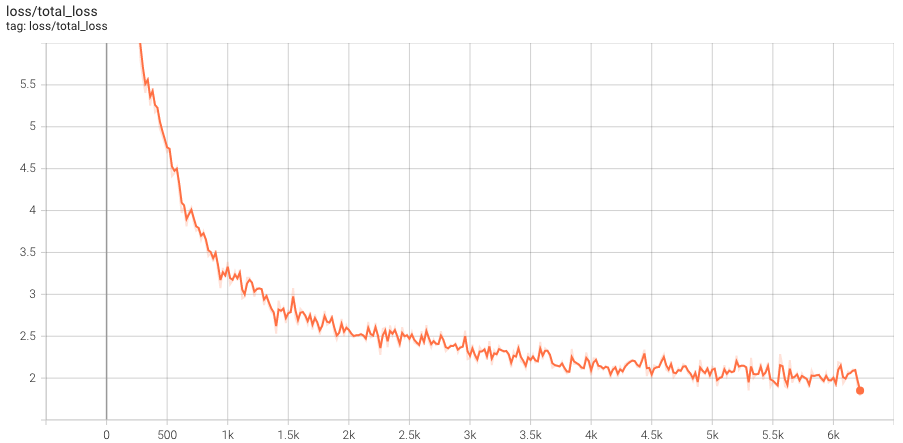
\includegraphics[width=\textwidth]{Images/task4b_total_loss.png}
        \caption*{Total loss during training}
    \end{subfigure}
    \hfill
    \begin{subfigure}[b]{\textwidth}
        \centering
        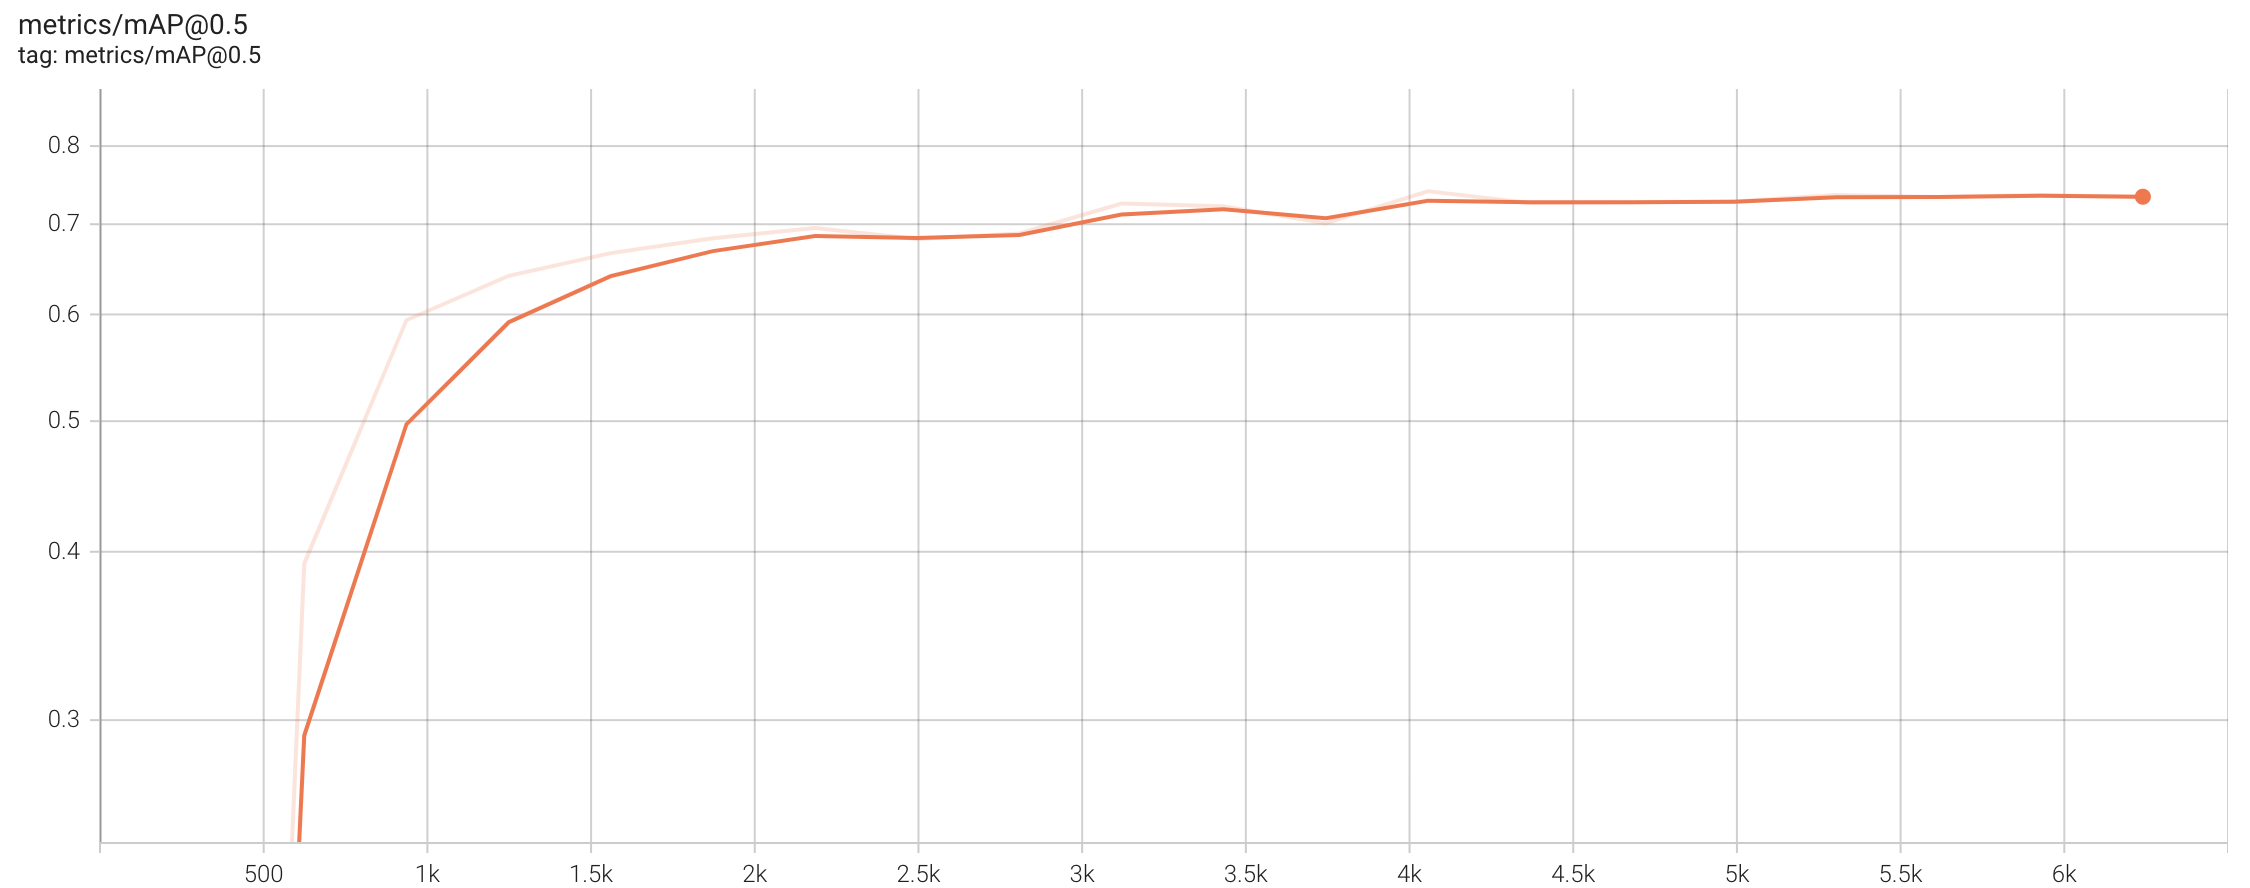
\includegraphics[width=\textwidth]{Images/task4b_map05.png}
        \caption*{mAP@0.5 during training}
    \end{subfigure}
\end{figure}

\clearpage
\subsection*{Task 4c}
Using the same logic from the last subtask, reaching a mean average precision before 10 000 iterations would mean a maximum of 32 epochs using a batch size of 32.
I started off changing the learning rate to $0.0026$ and changing the optimizer to Adam. This yielded some effect. 
In addition I changed the mean and std to the values recommended by PyTorch.
When running this I noticed that a problem was detecting smaller items, and I therefore halved the two smallest anchor boxes.
With these implementations I managed to get to 85-87\% already after 20 epochs, with only small changes to the layers.
I made multiple attempts at trying to add batch normalization and dropout to the model, without significant effect.
This only lead to the model having a harder time converging, and as I had already gotten 85\% I did not experiment any further with this.
The total loss and mAP@0.5 are shown below, and the final layer structure of the model are shown on the next page.

\begin{figure}[h!]
    \centering
    \begin{subfigure}[b]{\textwidth}
        \centering
        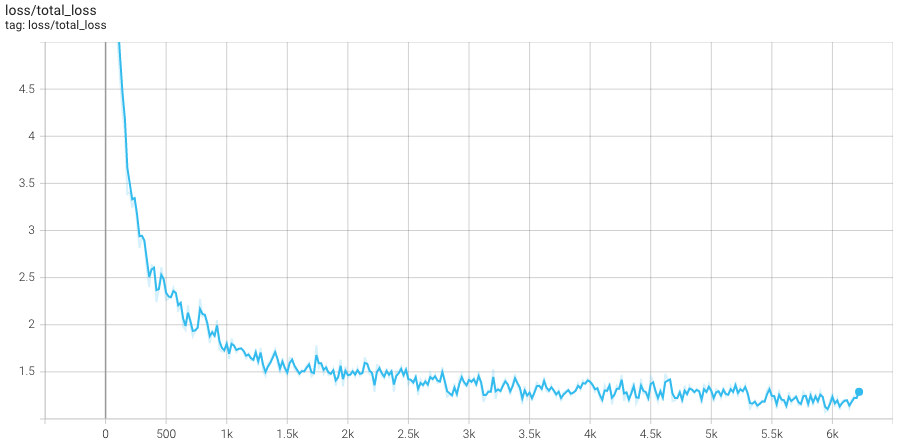
\includegraphics[width=\textwidth]{Images/task4c_total_loss.png}
        \caption*{Total loss during training}
    \end{subfigure}
    \hfill
    \begin{subfigure}[b]{\textwidth}
        \centering
        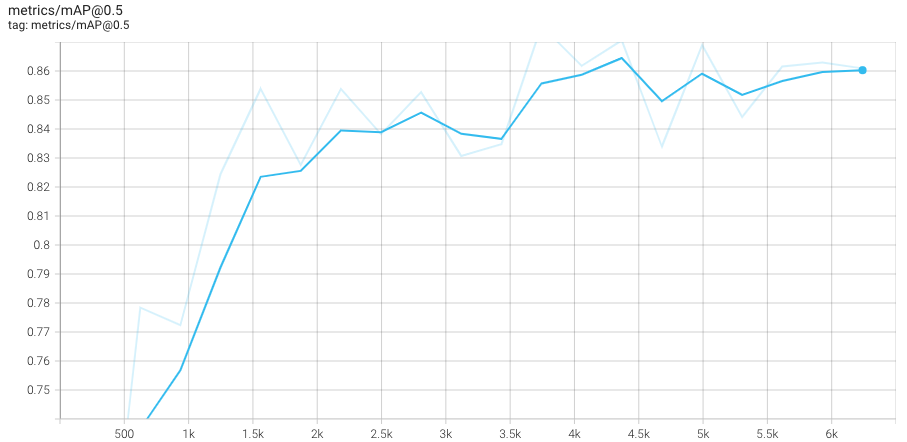
\includegraphics[width=\textwidth]{Images/task4c_map05.png}
        \caption*{mAP@0.5 during training}
    \end{subfigure}
\end{figure}

\clearpage
\begin{table}[h!]
    \centering
    \caption*{Important parameters in the config}
    \begin{tabular}{|l|l|}
        \hline \text { Learning rate } & 0.0026 \\
        \hline \text { Batch size } & 32 \\
        \hline \text { Epochs } & 32 \\
        \hline \text { Mean } & {[0.485, 0.456, 0.406]} \\
        \hline \text { Std } & {[0.229, 0.224, 0.225]} \\
        \hline \text { Out channels } & {[128, 256, 128, 128, 64, 64]} \\
        \hline \text { Aspect ratios } & {[15,15],[30,30],[111,111],[162,162],[213,213],[264,264],[315,315]} \\
        \hline \text { Weight decay } & 0.0005 \\
        \hline
    \end{tabular}
\end{table}

\begin{table}[h!]
    \centering
    \caption*{Model structure}
    \begin{tabular}{l|l|l|l}
        \hline 
        Is Output & Layer Type & Number of Filters & Stride \\
        \hline 
            & Conv2D & 32 & 1 \\
            & MaxPool2D & $-$ & 2 \\
            & ReLU & $-$ & $-$ \\
            & Conv2D & 64 & 1 \\
            & MaxPool2D & $-$ & 2 \\
            & ReLU & $-$ & $-$ \\
            & Conv2D & 64 & 1 \\
            & ReLU & $-$ & $-$ \\
            Yes - Resolution: $38 \times 38$ & Conv2D & output\_channels[0] & 2 \\
        \hline
            & ReLU & $-$ & $-$ \\
            & Conv2D & 256 & 1 \\
            & ReLU & $-$ & $-$ \\
            Yes - Resolution: $19 \times 19$ & Conv2D & output\_channels[1] & 2 \\
        \hline 
            & ReLU & $-$ & $-$ \\
            & Conv2D & 256 & 1 \\
            & ReLU & $-$ & $-$ \\
            Yes - Resolution: $10 \times 10$ & Conv2D & output\_channels[2] & 2 \\
        \hline 
            & ReLU & $-$ & $-$ \\
            & Conv2D & 256 & 1 \\
            & ReLU & $-$ & $-$ \\
            Yes - Resolution: $5 \times 5$ & Conv2D & output\_channels[3] & 2 \\
        \hline 
            & ReLU & $-$ & $-$ \\
            & Conv2D & 256 & 1 \\
            & ReLU & $-$ & $-$ \\
            Yes - Resolution: $3 \times 3$ & Conv2D & output\_channels[4] & 2 \\
        \hline 
            & ReLU & $-$ & $-$ \\
            & Conv2D & 256 & 1 \\
            & ReLU & $-$ & $-$ \\
            Yes - Resolution: $1 \times 1$ & Conv2D & output\_channels[5] & 2 \\
        \hline
    \end{tabular}
\end{table}

\clearpage
\subsection*{Task 4d}
In this task, we are to show the placement of anchor box centers, and calculate the size of the anchor boxes used for the feature map with 5x5 resolution, and 64x64 stride.

I started off by calculating the centers of each anchor box.
As the given feature map resolution is 5x5, we divide the 300x300px image into a grid of 5x5 tiles of size 64x64 because of the nature of striding.
Further on we know that the centre point is in centre of the tile and get that the first centre point is (32, 32).
Because of the 64x64 stride, we have that the next centre is 64px to the right at (32, 96).
This applies for both x and y direction. 
As you can see, even though the tiles go past the border of the image, the anchor centres is all located within the image frame, but a little shifted to the right border.
On the next page we calculate the anchor box sizes and visualize all anchor boxes.

\begin{figure*}[h!]
    \centering
    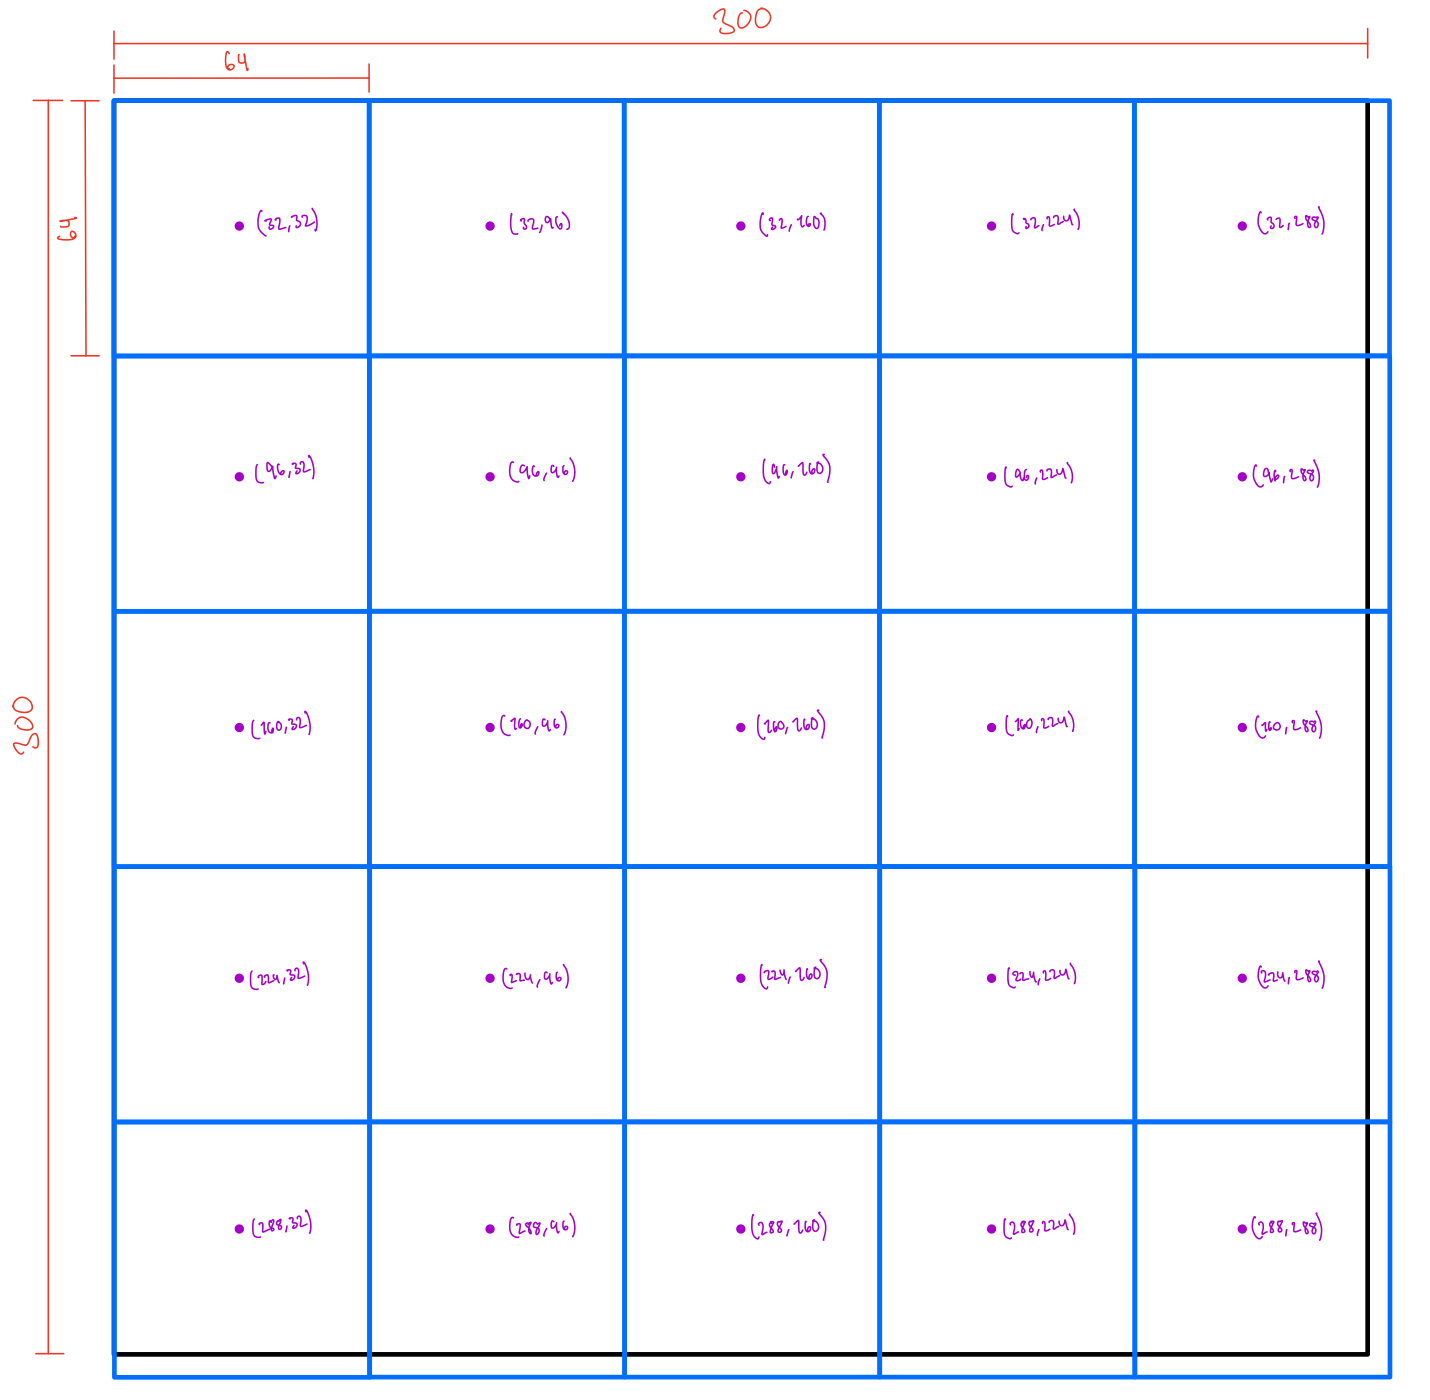
\includegraphics[width=\textwidth]{Images/task4d_illustration.png}
\end{figure*}

\clearpage
We continue with the task, where we are asked to find the 6 anchor box sizes used at each anchor box centre.
For calculating these, we are given 4 equations, where two of them are applied twice. These are:

\begin{itemize}
    \item $[\text{min\_size, min\_size}]$
    \item $[\sqrt{min\_size \cdot next\_min\_size}, \sqrt{min\_size \cdot next\_min\_size}]$
    \item $[min\_size$ $\cdot\; \sqrt{\text { aspect\_ratio1 }}$, $min\_size$ $/\; \sqrt{\text { aspect\_ratio1 }}]$
    \item $[min\_size$ $/\; \sqrt{\text { aspect\_ratio1 }}$, $min\_size$ $\cdot\; \sqrt{\text { aspect\_ratio1 }}]$
    \item $[min\_size$ $\cdot\; \sqrt{\text { aspect\_ratio2 }}$, $min\_size$ $/\; \sqrt{\text { aspect\_ratio2 }}]$
    \item $[min\_size$ $/\; \sqrt{\text { aspect\_ratio2 }}$, $min\_size$ $\cdot\; \sqrt{\text { aspect\_ratio2 }}]$
\end{itemize}

We solve them with aspect ratio $[2,3]$, $min\_size = 162$ and $next\_min\_size = 213$:
\begin{itemize}
    \item $[162, 162]$
    \item $[\sqrt{162 \cdot 213}, \sqrt{162 \cdot 213}] = [186, 186]$
    \item $[162\cdot\sqrt(2), 162/\sqrt(2)] = [229, 115]$
    \item $[162/\sqrt(2), 162\cdot\sqrt(2)] = [115, 229]$
    \item $[162\cdot\sqrt(3), 162/\sqrt(3)] = [281, 94]$
    \item $[162/\sqrt(3), 162\cdot\sqrt(3)] = [94, 281]$
\end{itemize}

This yields us 6 boxes per location, which can be confirmed in the notebook \newline
 \texttt{visualize\_priors.ipynb} as it it yields that there are to be 150 ($25 \cdot 6$) \newline 
 anchor boxes with 6 boxes per location.

\begin{figure}[h!]
    \centering
    \begin{subfigure}[b]{0.49\textwidth}
        \centering
        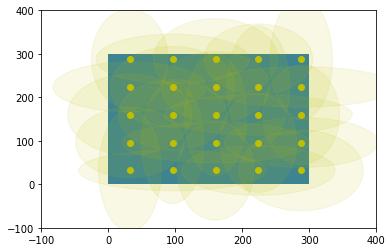
\includegraphics[width=\textwidth]{Images/task4d_plot_circles.png}
    \end{subfigure}
    \hfill
    \begin{subfigure}[b]{0.49\textwidth}
        \centering
        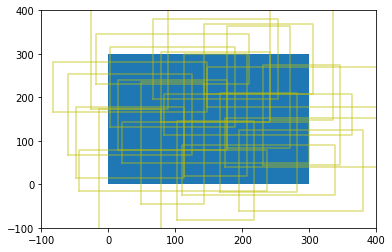
\includegraphics[width=\textwidth]{Images/task4d_plot_rectangles.png}
    \end{subfigure}
\end{figure}


\clearpage
\subsection*{Task 4e}

After running the command 
\begin{equation*}
    \texttt{python demo.py configs/task4e.py demo/mnist demo/mnist\_output}
\end{equation*}
I got the following labeled images

\begin{figure}[h!]
    \centering
    \begin{subfigure}[b]{0.193\textwidth}
        \centering
        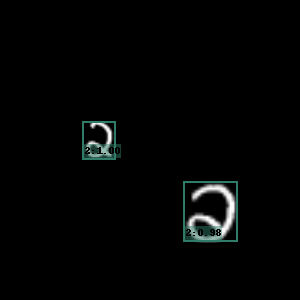
\includegraphics[width=\textwidth]{Images/mnist_output/0.png}
    \end{subfigure}
    \hfill
    \begin{subfigure}[b]{0.193\textwidth}
        \centering
        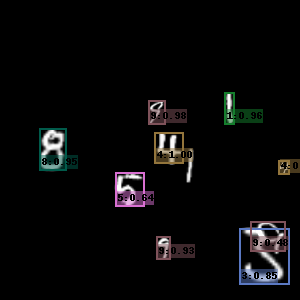
\includegraphics[width=\textwidth]{Images/mnist_output/1.png}
    \end{subfigure}
    \hfill
    \begin{subfigure}[b]{0.193\textwidth}
        \centering
        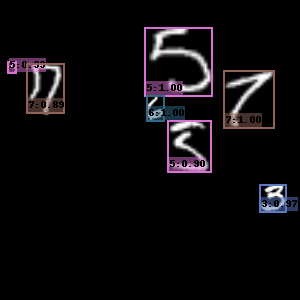
\includegraphics[width=\textwidth]{Images/mnist_output/2.png}
    \end{subfigure}
    \hfill
    \begin{subfigure}[b]{0.193\textwidth}
        \centering
        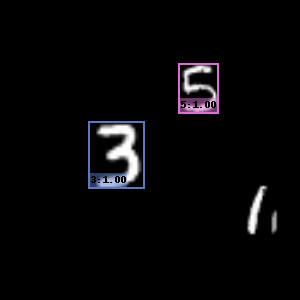
\includegraphics[width=\textwidth]{Images/mnist_output/3.png}
    \end{subfigure}
    \hfill
    \begin{subfigure}[b]{0.193\textwidth}
        \centering
        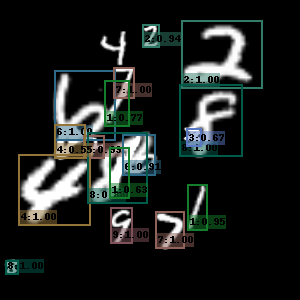
\includegraphics[width=\textwidth]{Images/mnist_output/4.png}
    \end{subfigure}
    \hfill
    \begin{subfigure}[b]{0.193\textwidth}
        \centering
        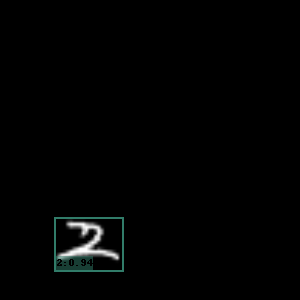
\includegraphics[width=\textwidth]{Images/mnist_output/5.png}
    \end{subfigure}
    \hfill
    \begin{subfigure}[b]{0.193\textwidth}
        \centering
        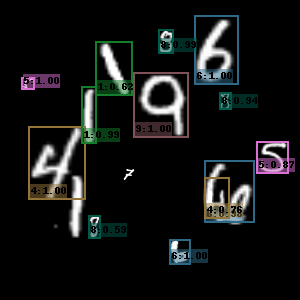
\includegraphics[width=\textwidth]{Images/mnist_output/6.png}
    \end{subfigure}
    \hfill
    \begin{subfigure}[b]{0.193\textwidth}
        \centering
        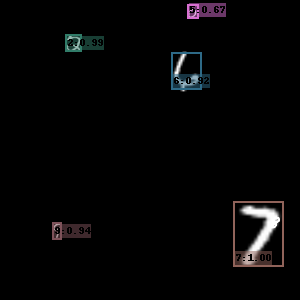
\includegraphics[width=\textwidth]{Images/mnist_output/7.png}
    \end{subfigure}
    \hfill
    \begin{subfigure}[b]{0.193\textwidth}
        \centering
        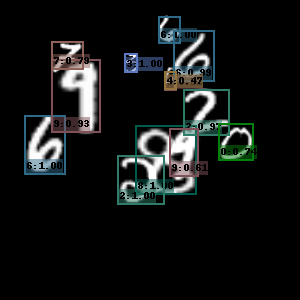
\includegraphics[width=\textwidth]{Images/mnist_output/8.png}
    \end{subfigure}
    \hfill
    \begin{subfigure}[b]{0.193\textwidth}
        \centering
        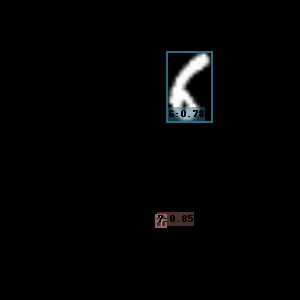
\includegraphics[width=\textwidth]{Images/mnist_output/9.png}
    \end{subfigure}
    \hfill
    \begin{subfigure}[b]{0.193\textwidth}
        \centering
        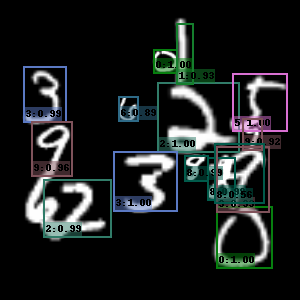
\includegraphics[width=\textwidth]{Images/mnist_output/10.png}
    \end{subfigure}
    \hfill
    \begin{subfigure}[b]{0.193\textwidth}
        \centering
        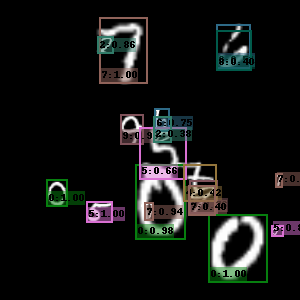
\includegraphics[width=\textwidth]{Images/mnist_output/11.png}
    \end{subfigure}
    \hfill
    \begin{subfigure}[b]{0.193\textwidth}
        \centering
        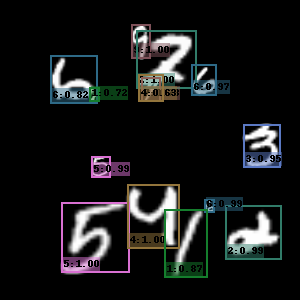
\includegraphics[width=\textwidth]{Images/mnist_output/12.png}
    \end{subfigure}
    \hfill
    \begin{subfigure}[b]{0.193\textwidth}
        \centering
        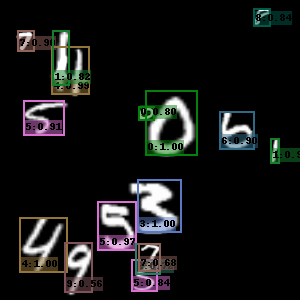
\includegraphics[width=\textwidth]{Images/mnist_output/13.png}
    \end{subfigure}
    \hfill
    \begin{subfigure}[b]{0.193\textwidth}
        \centering
        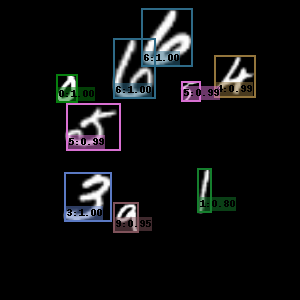
\includegraphics[width=\textwidth]{Images/mnist_output/14.png}
    \end{subfigure}
    \caption*{15 output images, labeled by a model with mAP@0.5 of 0.8734 on validation set}
\end{figure}

As you may observe from the images above, it seems like the number it have missed the most is the number 1.
In addition to this, it seems like some numbers are not recognized if they are located too close to other numbers.
Nevertheless, I would say this perform pretty good, and does confirm that the validation accuracy of 87.34\% is quite close to the performance in practice.

\clearpage
\subsection*{Task 4f}

In this task we were asked to train the VGG model provided in the handout code, on the PASCAL VOC dataset.
This was done by running the command

\begin{equation*}
    \texttt{python train.py configs/voc\_vgg.py}
\end{equation*}

As there was 256 batches, I ran the training for 20 epochs for a total of 5120 iterations.
After training for a little more than 5K iterations, the final validation mAP@0.5 was at 48.49\%.
The curves for total loss and mAP@0.5 are plotted below.

\begin{figure}[h!]
    \centering
    \begin{subfigure}[b]{\textwidth}
        \centering
        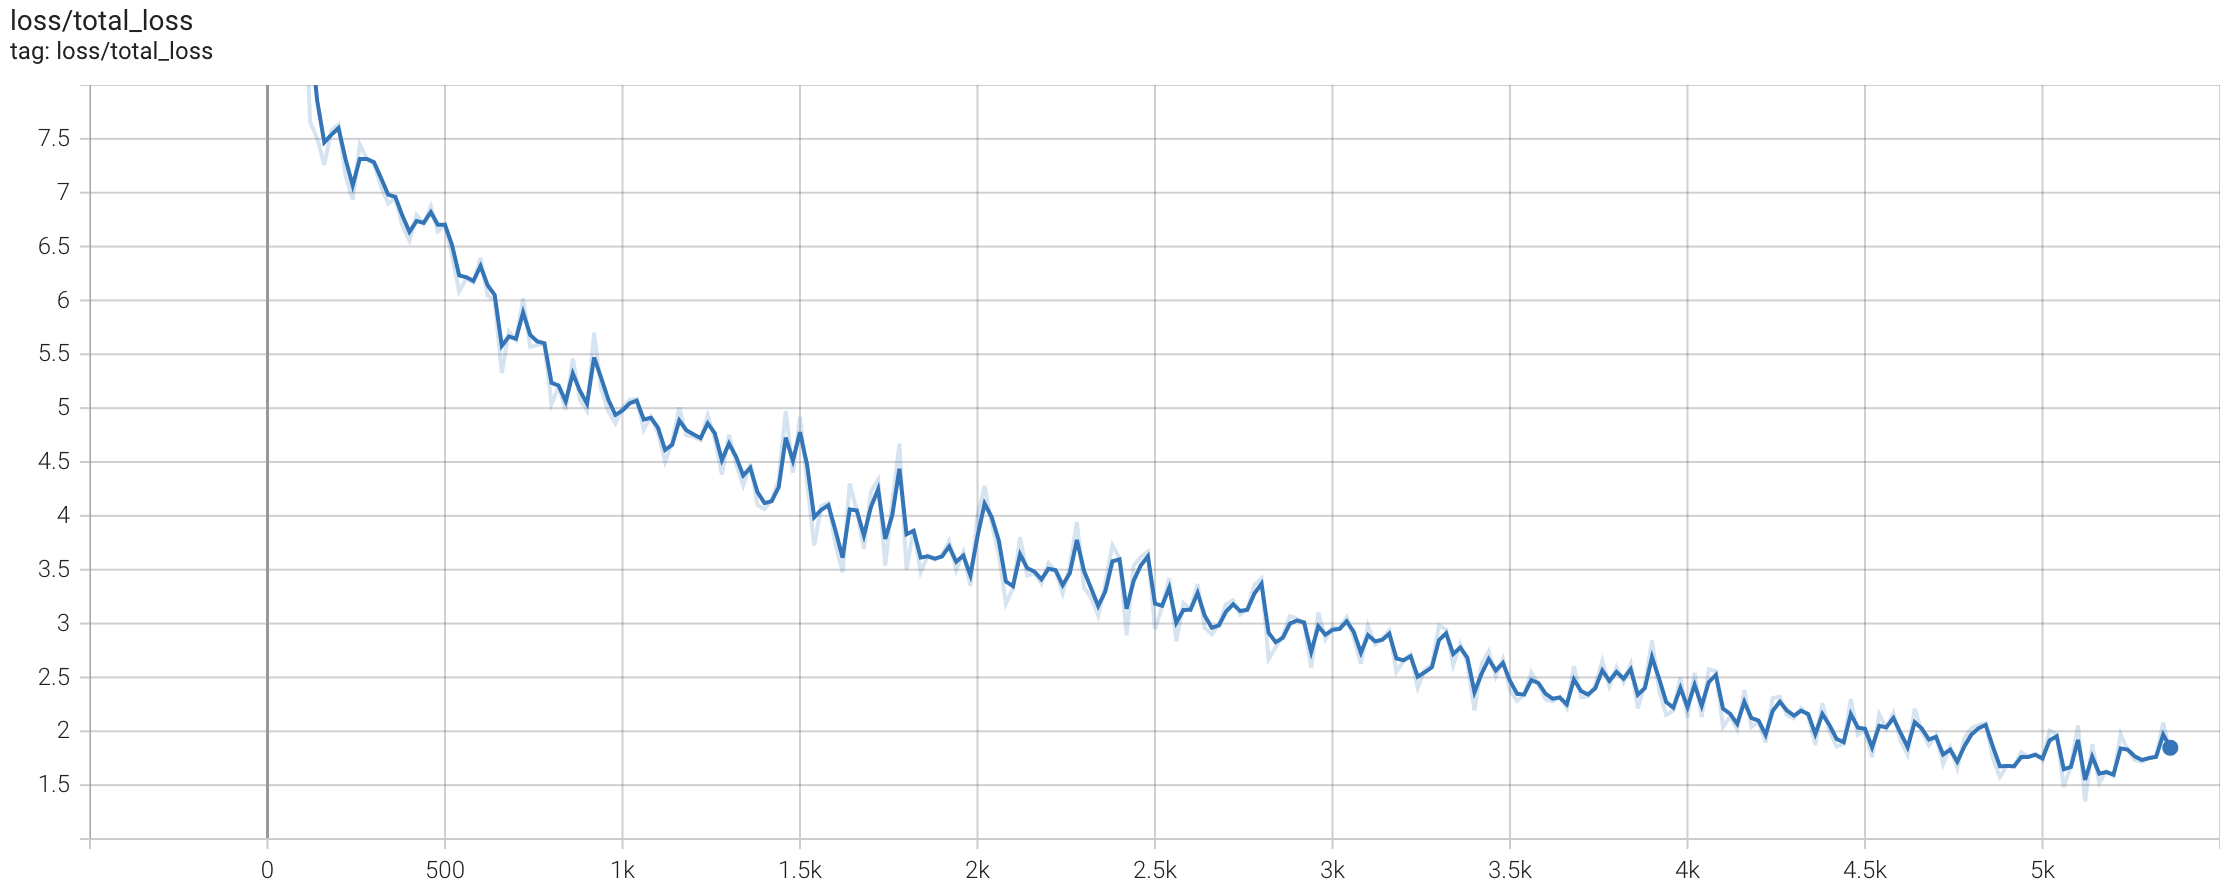
\includegraphics[width=\textwidth]{Images/task4f_total_loss.png}
        \caption*{Total loss during training}
    \end{subfigure}
    \hfill
    \begin{subfigure}[b]{\textwidth}
        \centering
        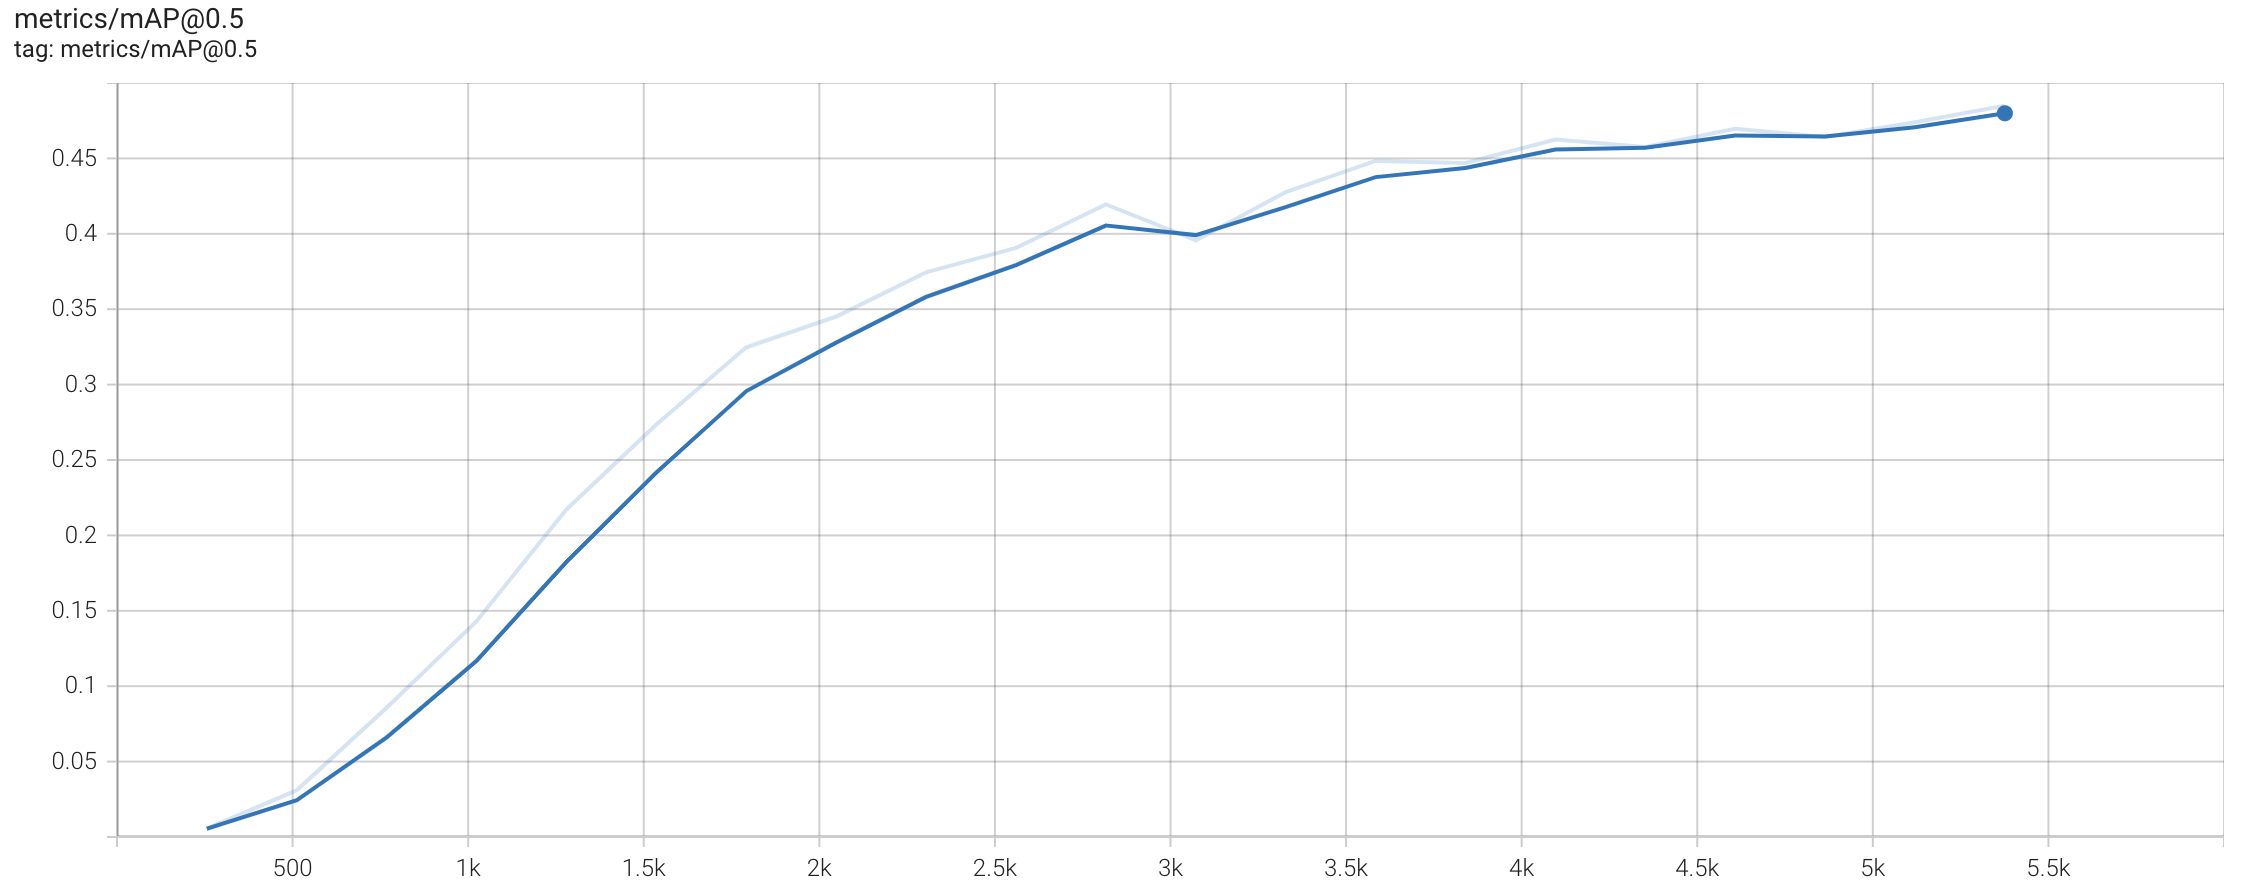
\includegraphics[width=\textwidth]{Images/task4f_map05.png}
        \caption*{mAP@0.5 during training}
    \end{subfigure}
\end{figure}


Further on, we were to test the model on a collection of 5 test-images. 
This was done by running the following command
\begin{equation*}
    \texttt{python demo.py configs/vog\_vgg.py demo/voc demo/voc\_output}
\end{equation*}
which yielded 5 labeled images. These can be found on the next page.
The model seems to be getting a lot of them correctly, 
almost better on the test-images than the precision of ~50\% would suggest.
Though, It should be mentioned that some objects are labeled completely wrong, overall a decent performance. 


\clearpage
\begin{figure}[h!]
    \centering
    \begin{subfigure}[b]{0.54\textwidth}
        \centering
        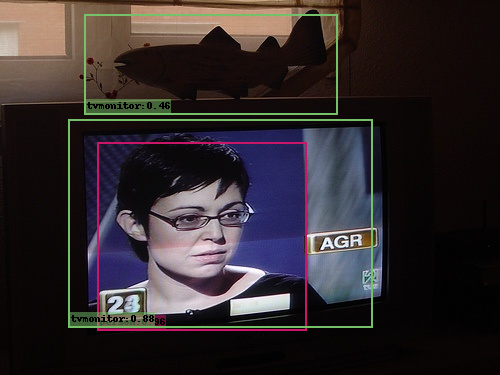
\includegraphics[width=\textwidth]{Images/voc_output/000342.png}
    \end{subfigure}
    \hfill
    \begin{subfigure}[b]{0.54\textwidth}
        \centering
        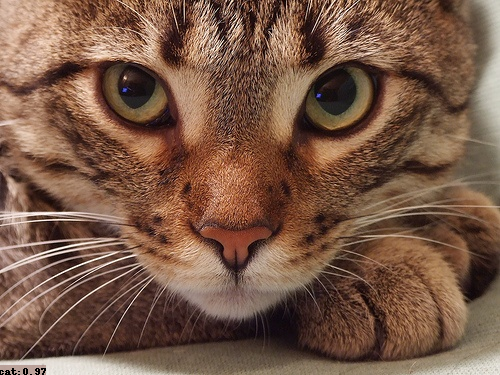
\includegraphics[width=\textwidth]{Images/voc_output/000542.png}
    \end{subfigure}
    \hfill
    \begin{subfigure}[b]{0.54\textwidth}
        \centering
        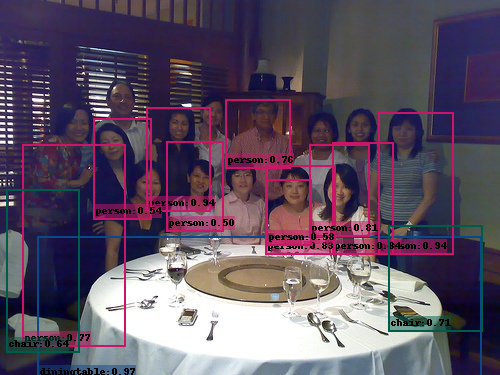
\includegraphics[width=\textwidth]{Images/voc_output/003123.png}
    \end{subfigure}
    \hspace{4cm}
    \begin{subfigure}[b]{0.28\textwidth}
        \centering
        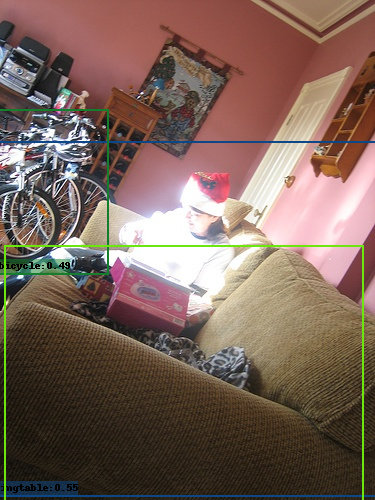
\includegraphics[width=\textwidth]{Images/voc_output/004101.png}
    \end{subfigure}
    \begin{subfigure}[b]{0.25\textwidth}
        \centering
        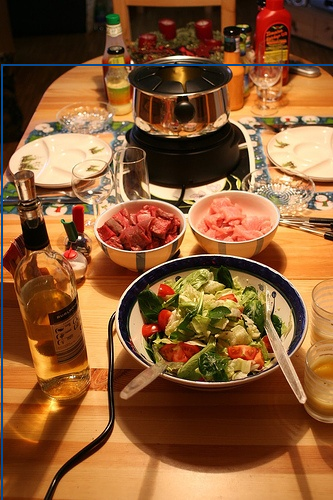
\includegraphics[width=\textwidth]{Images/voc_output/008591.png}
    \end{subfigure}
\end{figure}




